\section{MCA}
	\subsection{Study of Cs-137 spectrum and calculation of FWHM and resolution.}
		\begin{figure}[H]
			\centering
			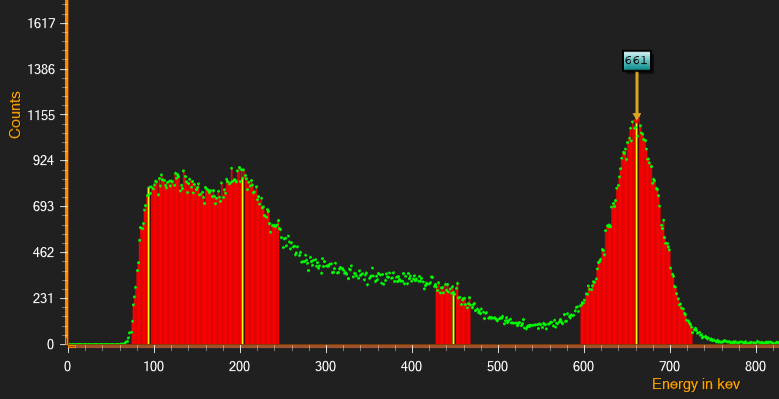
\includegraphics[width=0.9\columnwidth]{images/Cs.PNG}
			\caption{Cs-137 spectrum}
			\label{fig:cs}
		\end{figure}
		Table 6
		\begin{table}[H]
    \centering
    \begin{tabular}{|l|l|}
        \hline
        \textbf{Start}           & 398      \\ \hline
        \textbf{End}             & 512      \\ \hline
        \textbf{Number of Peaks} & 1        \\ \hline
        \textbf{Peak}            & 463.1764 \\ \hline
        \textbf{FW(C)}           & 46.8672  \\ \hline
        \textbf{TM/HM}           & 1.7803   \\ \hline
        \textbf{FM/HM}           & 2.1577   \\ \hline
        \textbf{Gross}           & 57839    \\ \hline
        \textbf{Net}             & 47546.5  \\ \hline
    \end{tabular}
    \caption{Cs-137 Peak Report}
    \label{tab:cs}
\end{table}
		from \hyperref[tab:cs]{Table 6} we have FWHM = $46.8672$

		Resolution is defined as the ratio of FWHM and peak channel.

		$$\fbox{resolution=7.21\%}$$
	\subsection{Energy calibration of gamma-ray spectrometer with energies of different Gamma Sources}
		Three different sources are placed in front of detector at once and spectrum is analysed to obtain the calibration curve.
		\begin{figure}[H]
			\centering
			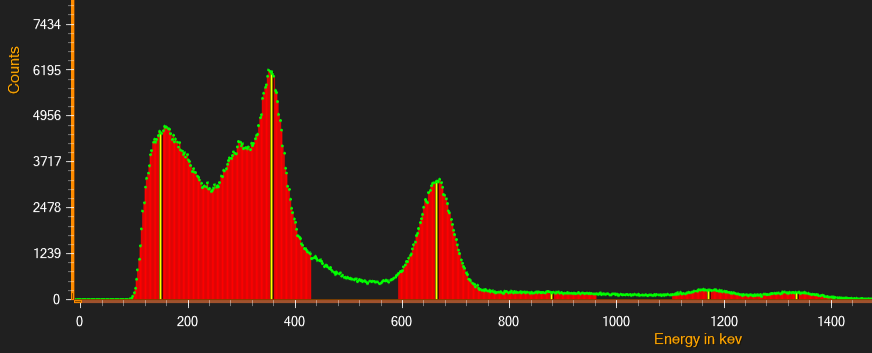
\includegraphics[width=0.9\columnwidth]{images/3mat.PNG}
			\caption{Ba-133, Cs-137 and Co-60 spectrum}
			\label{fig:3mat}
		\end{figure}
		Table 7\\
		\begin{table}[H]
    \centering
    \begin{tabular}{|l|l|l|l|l|}
    \hline
        Energy & Channel & FW (CH) & FW (EN) & ~ \\ \hline
        148.7619781 & 68 & 32.61084366 & 76.88145447 & ~ \\ \hline
        355.5156555 & 156 & 31.41841316 & 73.56323242 & ~ \\ \hline
        663.1218872 & 288.0596924 & 30.29399109 & 70.19688416 & ~ \\ \hline
        877.6900635 & 381 & 36.08543777 & 83.00172424 & ~ \\ \hline
        1170.310425 & 508.8700256 & 28.70510101 & 65.35279083 & ~ \\ \hline
        1336.052124 & 581.8839111 & 29.6067009 & 67.00904083 & ~ \\ \hline
        2253.693115 & 994.2141724 & 15 & 32.81540298 & ~ \\ \hline
    \end{tabular}
\end{table}
		\begin{figure}[H]
			\centering
			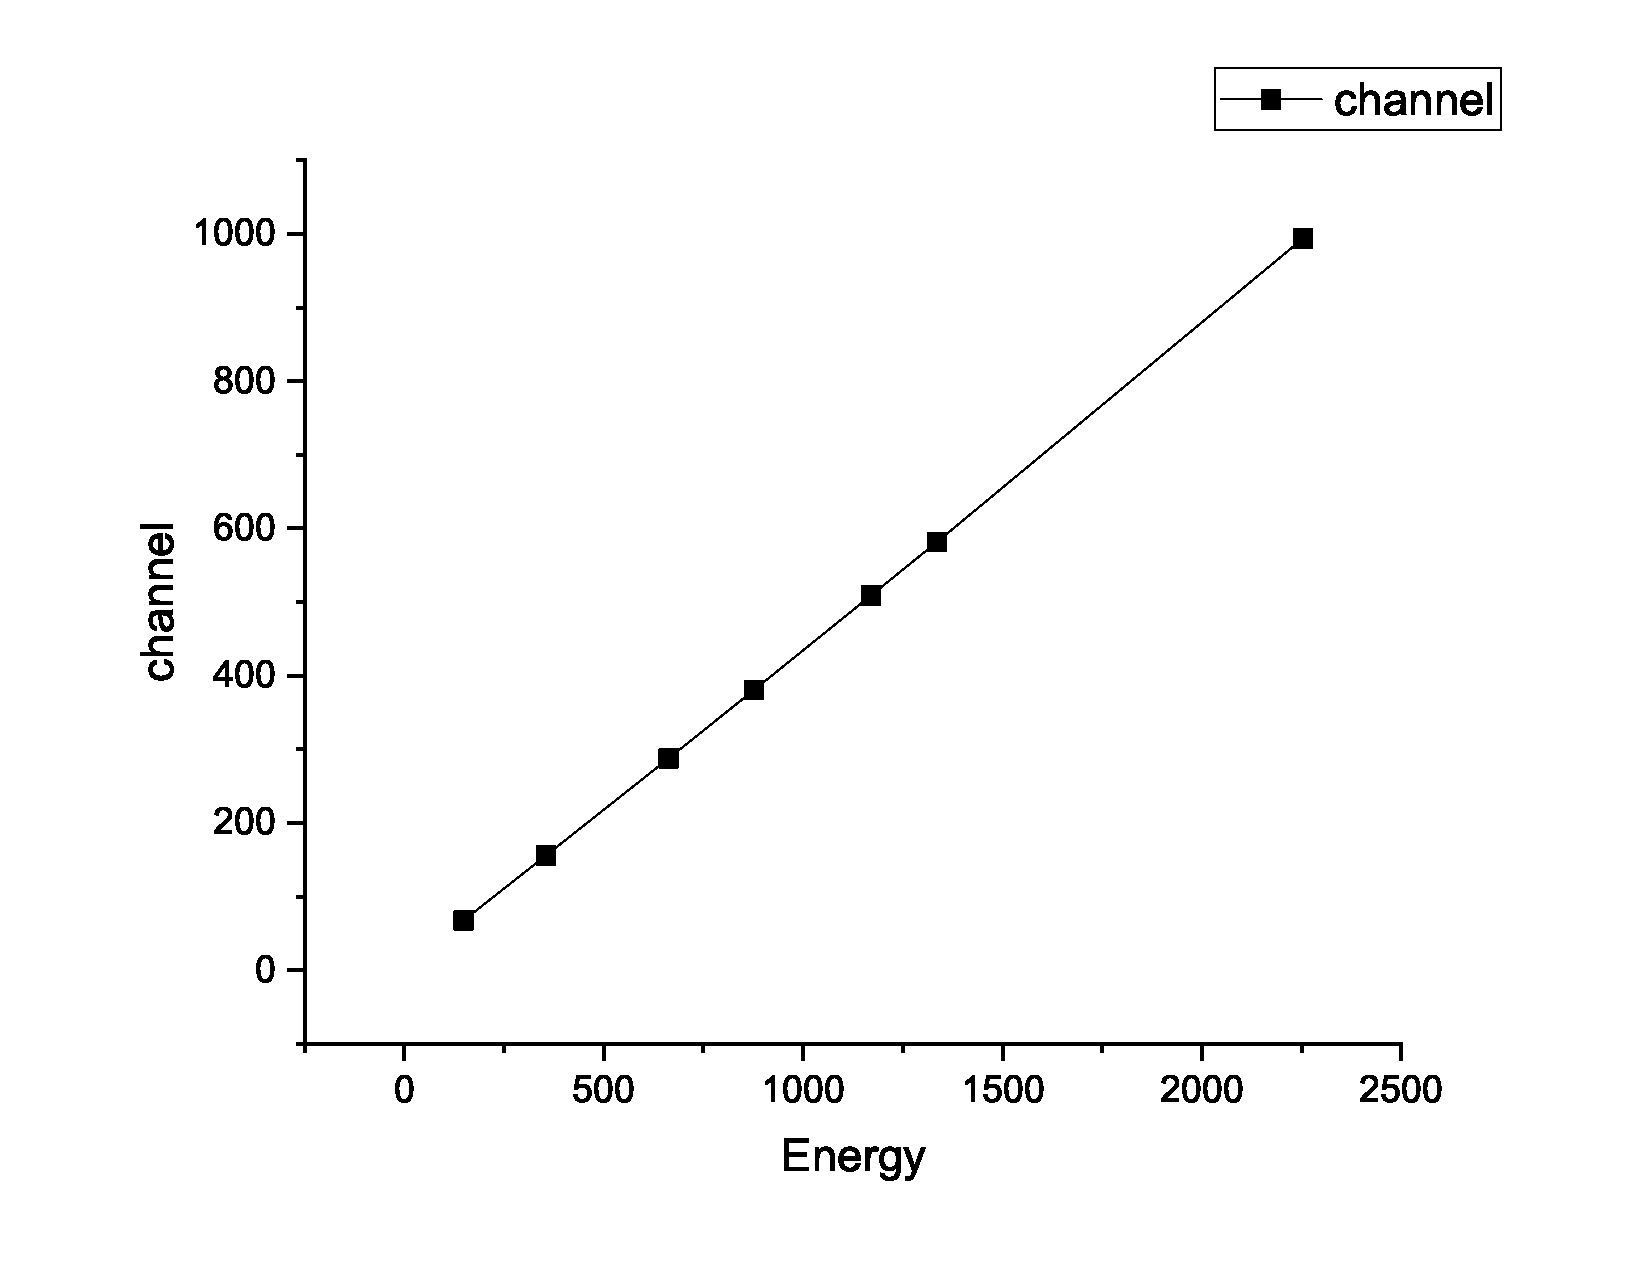
\includegraphics[width=0.9\columnwidth]{images/graph7.eps}
			\caption{Energy calibration curve}
		\end{figure}
	\subsection{Find of energy of Na-22 source}
		\begin{figure}[H]
			\centering
			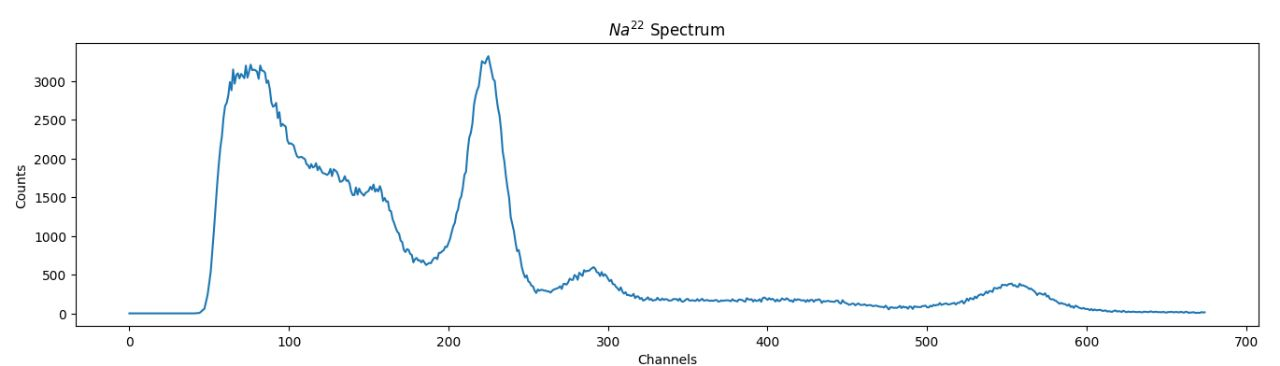
\includegraphics[width=0.9\columnwidth]{images/na.PNG}
			\caption{Na-22 spectrum}
		\end{figure}
		\begin{table}[H]
    \centering
    \begin{tabular}{|l|l|l|l|}
    \hline
        Type & Channel & FW (CH) & ~ \\ \hline
        M & 62.64506912 & 15 & ~ \\ \hline
        m & 81.37265778 & 15 & ~ \\ \hline
        M & 130.0105743 & 15 & ~ \\ \hline
        m & 157.321991 & 16.27744293 & ~ \\ \hline
          & 223.8300934 & 24.70108604 & ~ \\ \hline
          & 290.2333069 & 25.82227325 & ~ \\ \hline
        M & 408.0601807 & 35.67868042 & ~ \\ \hline
        m & 435 & 15 & ~ \\ \hline
          & 554.2346191 & 44.66348267 & ~ \\ \hline
          & 787.3337402 & 35.91174316 & ~ \\ \hline
          & 990 & 59.86914444 & ~ \\ \hline
    \end{tabular}
\end{table}
		From 8 and the energy calibration curve, we find that Na-22 has peak energies at 500KeV(ch-223),680 keV(ch-290), 1220KeV(Ch-554).
	\subsection{Mass absorption coefficient of Al}
		For 662 keV gamma rays, the mass absorption coefficient of Al is measured by placing aluminum blocks of different thicknesses between the detector and the source.\\
		\begin{table}[H]
    \centering
    \begin{tabular}{|l|l|}
    \hline
        Thickness(cm) & Count \\ \hline
        0 & 3560 \\ \hline
        0.5 & 1633 \\ \hline
        1 & 1218 \\ \hline
        1.5 & 950 \\ \hline
        2 & 815 \\ \hline
        2.5 & 750 \\ \hline
        3 & 615 \\ \hline
    \end{tabular}
\end{table}
		\begin{figure}[H]
			\centering
			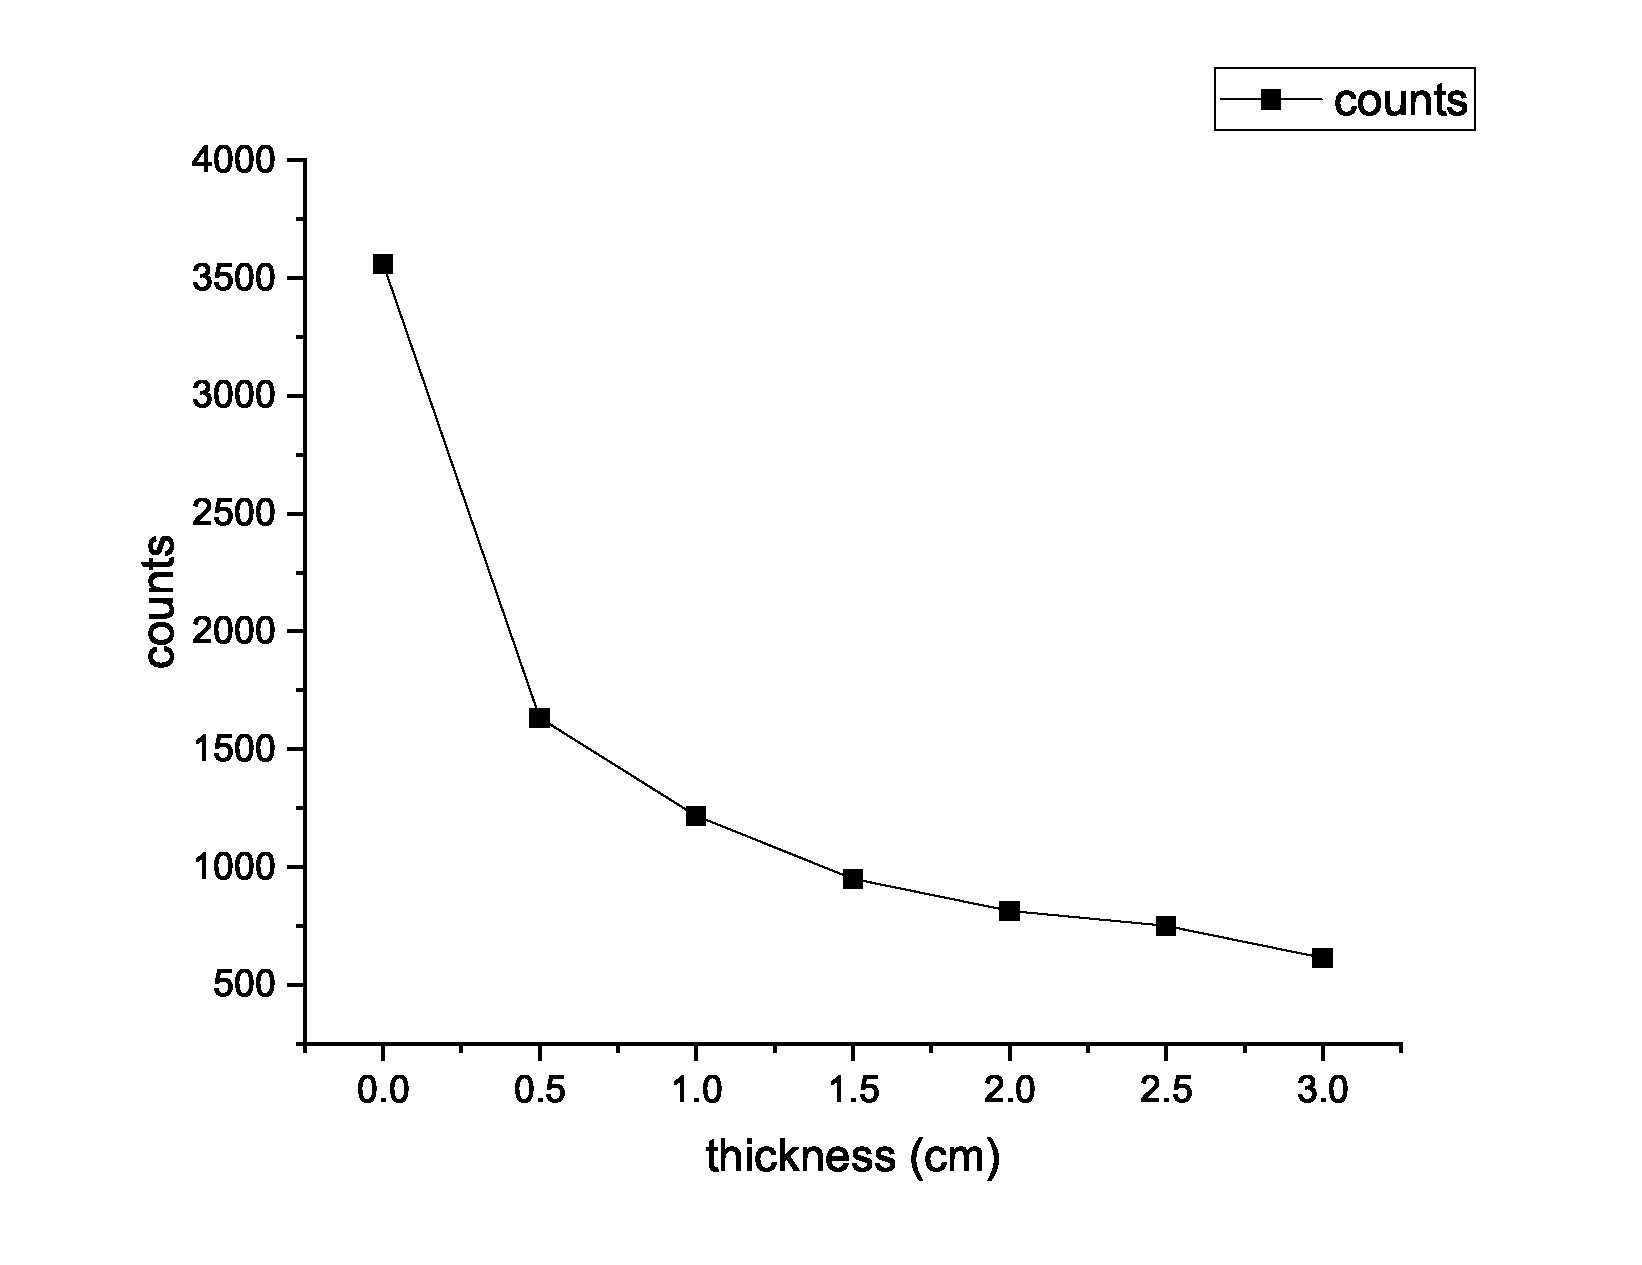
\includegraphics[width=0.9\columnwidth]{images/Graph6.eps}
			\caption{Absorption curve}
		\end{figure}
		From the graph Observed value of HVL (thickness at which counts are reduced to half) is 0.4cm.\\
		Density thickness=\(0.4\times 2.7gm/cm^3 =1.08gm/cm^2\)\\
		the mass absorption coefficient,\\
		m=\(\frac{0.693}{1.08} =0.641gm/cm^2\)